\documentclass{IEEEtran}
\usepackage{graphicx}
\usepackage{amssymb}
\usepackage{amsmath}
\usepackage[english]{babel}
\usepackage{cite}
\usepackage{float}
\usepackage{pgfgantt}
\usepackage{kantlipsum}
\usepackage{pdfpages}
\usepackage{fancyhdr}
\title {\author{ Josh Rendon, Micah Thornton} Proposal for Quantum Reversible Synthesis}
\pagestyle{fancy}


\begin{document}
\maketitle{}
\begin{abstract}
In this work we intend to create a design flow including development of a synthesis tool to determine if a classical circuit expressed as a Verilog module expresses a mathematically bijective function by expressing it as a quantum cascade of Toffoli gates.
Our proposed synthesis tool is based off the work of Fazel et al. \cite{4313212} which given a ESOP representation of a circuit as a cube list will produce a quantum cascade. 
\end{abstract}
\section{problem definition}
There are a number of classical circuits that benefit from the property of being a mathematical bijection. 
For instance a hash function necessarily needs to be a mathematical bijection in order to ensure there are no collisions in the mapping from inputs to hash outputs. 
Unfortunately, computationally efficient methods to determine if a circuit is in fact a bijection do not currently exist.
We propose the implementation of a software synthesis tool based on current work in the literature to determine if a classical circuit is a mathematical bijection.
If this circuit is synthesizable as a quantum cascade with no garbage outputs and no ancillia inputs then we know the circuit is logically reversible and is a bijection.
\section{Motivation}
All quantum circuits are known to be logically reversible, and hence bijections by their very nature. 
Our project hopes to exploit this feature of quantum circuits, and thereby through the synthesis of classical RTL, determine whether a boolean function is logically reversible. 
Consider the following example, imagine a 4-variable boolean function given by: 

\begin{table}[h!]
\caption{Truth Table for 4-bit circular hash function}
\begin{center}
\begin{tabular}{| c  c  c  c | c  c  c  c |}
    \hline
    in$_1$&in$_2$&in$_3$&in$_4$&out$_1$&out$_2$&out$_3$ & out$_4$ \\
    \hline
    \hline
    0&0&0&0&0&0&0&1 \\
    0&0&0&1&0&0&1&0 \\
    0&0&1&0&0&0&1&1 \\
    0&0&1&1&0&1&0&0 \\ 
    0&1&0&0&0&1&0&1 \\ 
    0&1&0&1&0&1&1&0 \\ 
    0&1&1&0&0&1&1&1 \\ 
    0&1&1&1&1&0&0&0 \\ 
    1&0&0&0&1&0&0&1 \\ 
    1&0&0&1&1&0&1&0 \\ 
    1&0&1&0&1&0&1&1 \\ 
    1&0&1&1&1&1&0&0 \\ 
    1&1&0&0&1&1&0&1 \\ 
    1&1&0&1&1&1&1&0 \\ 
    1&1&1&0&1&1&1&1 \\
    1&1&1&1&0&0&0&0 \\ 
    \hline
\end{tabular}
\end{center}

\end{table}

This hash function is considered circular, because it is based on a Caeser cipher, which rotates a character by one lexicographical position. 
The Boolean functions given by the truth table are specified below: 

\begin{align}
    out_1& = in_1 \oplus in_3in_2in_1\\
    out_2& = in_2 \oplus in_3in_2\\
    out_3& = in_3 \oplus in_3 \\
    out_4& = \overline{in_4} 
\end{align}

The corresponding classical circuit schematic for these equations is shown below: 

\begin{figure}[h!]
\begin{center}
\textit{\small{Figure 1: Classical Circuit Schematic for 4-bit Circular Hash}}
  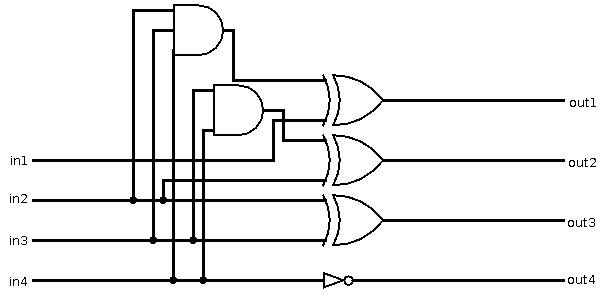
\includegraphics[scale=0.35]{figures/fbch.png}
\end{center}
\end{figure}

Because this Boolean function is fully specified for all possible values in the domain, we say it is injective. And because all values in the range of the function are mapped onto by the domain, we say it is surjective. A bijection by definition is both injective and surjective, therefore this function is a bijection, and should result in a quantum cascade without any ancilla or garbage bits required. The following figure represents a manually synthesized quantum cascade specifying the 4-bit circular hash function. 
One can see that this circuit requires no ancilla inputs or garbage outputs therefore is a mathematically bijective function. 

\begin{figure}[h!]
\begin{center}
\textit{\small{Figure 2: Quantum Cascade for 4-bit Circular Hash}} 
  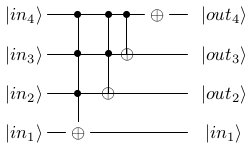
\includegraphics[scale=0.6]{figures/4-bit_circular_hash_qc.png}
\end{center}
\end{figure}

In contrast, consider another example this time, a classical full-adder. The truth table is specified below: 

\begin{table}[h!]
\caption{Truth Table for Full-adder}
\begin{center}
\begin{tabular}{| c  c | c  c |}
    \hline
    a&b&s&c \\
    \hline
    \hline
    0&0&0&0 \\
    0&1&1&0 \\
    1&0&1&0 \\
    1&1&0&1 \\ 
    \hline
\end{tabular}
\end{center}

\end{table}

The classical circuit represented by this truth table is diagrammed in Figure 3.

\begin{figure}[h!]
\begin{center}
\textit{\small{\label{fig:cfa}Figure 3: Classical Circuit Schematic for a Full-Adder}}
  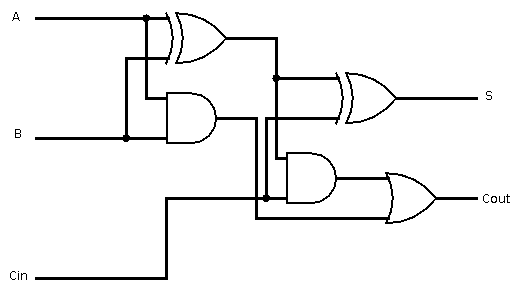
\includegraphics[scale=0.4]{figures/fulladder.png}
\end{center}
\end{figure}

To identify if the circuit was logically reversible we examined the quantum cascade for a full-adder as shown in \cite{qcagi}. It has been recreated below in Figure 4.

\begin{figure}[H]
\begin{center}
\textit{\small{\label{fig:qfa}Figure 4: Quantum Cascade for Full-Adder}} 
  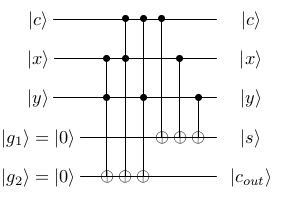
\includegraphics[scale=0.6]{figures/Full_adder_qc.png}
\end{center}
\end{figure}


This circuit demonstrates the fact that: if a circuit is not logically reversible, then an equivalent quantum cascade cannot be created without the addition of garbage output bits, or ancilla input bits.
The previous two circuits stand as examples of the soundness of the theoretical basis for our project. In the next section we will describe our intended design schedule, milestones and methods. 

\section{method}
We plan to accomplish three main tasks within the scope of this project. 
The first task is to design several Verilog hash circuits that will be used to test the synthesis tool.
Secondly we will design a synthesis tool in C or C++ that given a truth table of a circuit, or some equivalent form will generate the exclusive sum of products form for the minterms of the circuit.
Lastly, we plan to generate a visual representation of the cascade by adding functionality to the qasm tool developed by Neilson and Chaung. \cite{qasm2circ} 
In order to achieve our desired goal of producing a quantum cascade with no garbage outputs and no ancilla inputs for logically reverisble circuits, 
In order to achieve these goals in addition to our synthesis tool, will need to use existing RTL simulation and synthesis tools like Cadence simvision, Design Compiler, and the EXORCISM ESOP minimizer tool\cite{exorcism}. 
For a full list of our milestones, and intended schedule see Appendix A, which includes a Gantt chart. 

\section{previous work}
This project is based mainly on the previous work of Fazel et al. \cite{4313212} It focuses on using an internal representation of a truth table that can be used to easily convert a classical circuit to an equivalent quantum cascade. 

\bibliography{quant_pro}{}
\bibliographystyle{IEEEtran}


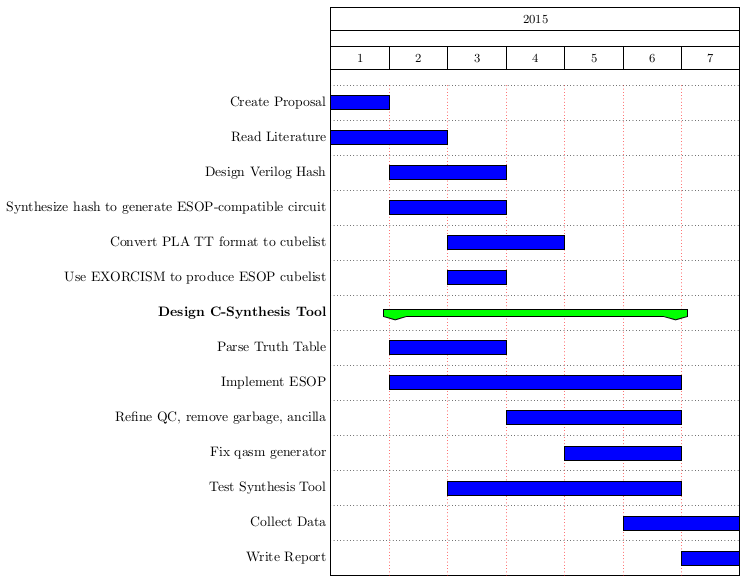
\includepdf[pages=1-,pagecommand={\thispagestyle{article}}]{our_gantt.pdf}


\end{document}

